\documentclass[twoside]{article}
\setlength{\oddsidemargin}{0.25 in}
\setlength{\evensidemargin}{-0.25 in}
\setlength{\topmargin}{-0.6 in}
\setlength{\textwidth}{6.5 in}
\setlength{\textheight}{8.5 in}
\setlength{\headsep}{0.75 in}
\setlength{\parindent}{0 in}
\setlength{\parskip}{0.1 in}


\usepackage{graphicx}
\usepackage{url}

%
% The following commands sets up the lecnum (lecture number)
% counter and make various numbering schemes work relative
% to the lecture number.
%
\newcounter{lecnum}
\renewcommand{\thepage}{\thelecnum-\arabic{page}}
\renewcommand{\thesection}{\thelecnum.\arabic{section}}
\renewcommand{\theequation}{\thelecnum.\arabic{equation}}
\renewcommand{\thefigure}{\thelecnum.\arabic{figure}}
\renewcommand{\thetable}{\thelecnum.\arabic{table}}
\newcommand{\dnl}{\mbox{}\par}

%
% The following macro is used to generate the header.
%
\newcommand{\lecture}[4]{
  \pagestyle{myheadings}
  \thispagestyle{plain}
  \newpage
  \setcounter{lecnum}{#1}
  \setcounter{page}{1}
  \noindent
  \begin{center}
  \framebox{
     \vbox{\vspace{2mm}
   \hbox to 6.28in { {\bf COMPSCI~630~~~Systems
                       \hfill Spring 2017} }
      \vspace{4mm}
      \hbox to 6.28in { {\Large \hfill Lecture #1: #2  \hfill} }
      \vspace{2mm}
      \hbox to 6.28in { {\it Lecturer: #3 \hfill Scribe(s): #4} }
     \vspace{2mm}}
  }
  \end{center}
  \markboth{Lecture {#1}: #2}{Lecture {#1}: #2}
  \vspace*{4mm}
}

%
% Convention for citations is authors' initials followed by the year.
% For example, to cite a paper by Leighton and Maggs you would type
% \cite{LM89}, and to cite a paper by Strassen you would type \cite{S69}.
% (To avoid bibliography problems, for now we redefine the \cite command.)
%
\renewcommand{\cite}[1]{[#1]}

% \input{epsf}

%Use this command for a figure; it puts a figure in wherever you want it.
%usage: \fig{NUMBER}{FIGURE-SIZE}{CAPTION}{FILENAME}
\newcommand{\fig}[4]{
           \vspace{0.2 in}
           \setlength{\epsfxsize}{#2}
           \centerline{\epsfbox{#4}}
           \begin{center}
           Figure \thelecnum.#1:~#3
           \end{center}
   }

% Use these for theorems, lemmas, proofs, etc.
\newtheorem{theorem}{Theorem}[lecnum]
\newtheorem{lemma}[theorem]{Lemma}
\newtheorem{proposition}[theorem]{Proposition}
\newtheorem{claim}[theorem]{Claim}
\newtheorem{corollary}[theorem]{Corollary}
\newtheorem{definition}[theorem]{Definition}
\newenvironment{proof}{{\bf Proof:}}{\hfill\rule{2mm}{2mm}}

% Some useful equation alignment commands, borrowed from TeX
\makeatletter
\def\eqalign#1{\,\vcenter{\openup\jot\m@th
 \ialign{\strut\hfil$\displaystyle{##}$&$\displaystyle{{}##}$\hfil
     \crcr#1\crcr}}\,}
\def\eqalignno#1{\displ@y \tabskip\@centering
 \halign to\displaywidth{\hfil$\displaystyle{##}$\tabskip\z@skip
   &$\displaystyle{{}##}$\hfil\tabskip\@centering
   &\llap{$##$}\tabskip\z@skip\crcr
   #1\crcr}}
\def\leqalignno#1{\displ@y \tabskip\@centering
 \halign to\displaywidth{\hfil$\displaystyle{##}$\tabskip\z@skip
   &$\displaystyle{{}##}$\hfil\tabskip\@centering
   &\kern-\displaywidth\rlap{$##$}\tabskip\displaywidth\crcr
   #1\crcr}}
\makeatother

% **** IF YOU WANT TO DEFINE ADDITIONAL MACROS FOR YOURSELF, PUT THEM HERE:

% Some general latex examples and examples making use of the
% macros follow.

\begin{document}

%FILL IN THE RIGHT INFO.
%\lecture{**LECTURE-NUMBER**}{**DATE**}{**LECTURER**}{**SCRIBE**}
\lecture{9}{Networking}{Emery Berger}{Andrew Danise, Jayanth Hegde}
\section{LAN Architecture}

We reviewed point-to-point, ring, and daisy chain networks.
Our discussion focused on how the number of connections used
in these networks provide a tradeoff between fault tolerance
and network cost.

Early network communication between computer systems was through point-to-point full connections. This requires a lot
of wiring. Thus, several network topologies are used to connect all systems in a network. These topologies do
not require all systems to be connected to each other but as a trade-off may cause partition when a main connection
such as a bus is broken.

Some example topologies: Mesh (fully connected same as the naive connection topology described above), Ring, Daisy chain,
Star, Bus or backbone, Tree etc.

\subsection{Partition Tolerance}
We used partition tolerance as a metric to describe the fault
tolerance of a network. Partition tolerance is the minimum
number of failures a network can sustain before some portion
of the network can no longer communicate with another portion.

\subsection{Point to Point}
In a point to point network, each system is directly connected
to every other system in the network. Given a network with $N$
nodes, the number of connections in the network is
$\frac{N(N-1)}{2}$. This network provides the strongest
possible fault tolerance without redundant connections. It has
a partition tolerance of $N$.

\subsection{Ring}
In a ring network, each system is directly connected to two
other systems in the network. Given a network with $N$ nodes, the
number of connections in the network is $N$. This network provides
weak fault tolerance. It has a partition tolerance of $2$.

\subsection{Daisy Chain}
A daisy chain network is similar to a ring network except one
the connections is removed. Given a network with $N$ nodes, this
topology requires only $N-1$ connections. The downside is that
it has extremely poor fault tolerance. It has a partition
tolerance of $1$.

\section{Internet Protocols}

We reviewed the UDP and TCP internet protocols.

\subsection{UDP}

UDP or User Datagram Protocol is a simple protocol for
transmitting data over a network. It does not try to provide any
guarantees about data sent over the network. It is an unreliable
protocol meaning it does not guarantee that data actually arrives
at its destination. It is also an out of order protocol which
means that data can arrive at the destination in a different order
than the order it was sent in. The UDP protocol is useful for
applications where data is only useful for a small window of time. One
example is streaming video. While streaming video, you will not notice
if a single frame of the video is dropped as long as most arrive on time.

\subsection{TCP}

TCP or Transmission Control Protocol is a packet based protocol designed
to provide reliable transmission of data over a network. In TCP, each packet
pecifies the transmission of a single payload of data. Every packet is
composed of two parts: a header and a payload. The header contains
metadata required to reliably send the packet over the network including
the sender, the recipient, the number of the packet, and a checksum to
verify the data was sent correctly. The payload is the data being sent.
In the TCP protocol, the sender sends a packet to the receiver. If the
receiver gets the packet it uses the checksum in the packet header to
verify the information. If everything checks out, then the receiver
sends an ACK back to the sender. If everything does not check
out, then the receiver sends a NACK back to the sender, informing
the sender that it needs to resend the data. It is also possible that
packets may never reach the receiver (or sender) in which case the sender
will retry the message after some timeout has elapsed.

\section{Packet switching and Virtual Circuits}

Method of communication in internet: In a network, communication between two systems occurs through passing of packets. This
is referred to as packet switching. 

Packet switching in a virtual circuit: A virtual circuit is an abstract circuit established in a network for the purpose of 
communication. A packet follows a particular path defined by the circuit in this type of communication. This allows packets to
reach reliably in an order. TCP is an example of a protocol that uses this type of communication. However, virtual circuit 
violates the goal of fault tolerance.

Also, virtual circuits do not provide anonymity and security. But it must be remembered that these were not original goals of 
Internet design.

Original goals of Internet design: Building a resilient, cost-effective communication system for military.

There is also a concept of accountability(tracking the load on our system created by foreign entities). This handled by switches.

An alternative method of communication is to use datagrams. These are used by protocols such as UDP. This method does not guarantee
ordered delivery of packets but it guarantees speedy delivery of packets to destination. At the destination, packets are ordered.
This is necessary when real time service is required.

\section{Packet Structure}
Consists of a header that contains sender and reciever addresses, sequence number(for TCP and other connection-oriented protocols)
and a data payload.

\begin{figure}[tph!]
\centerline{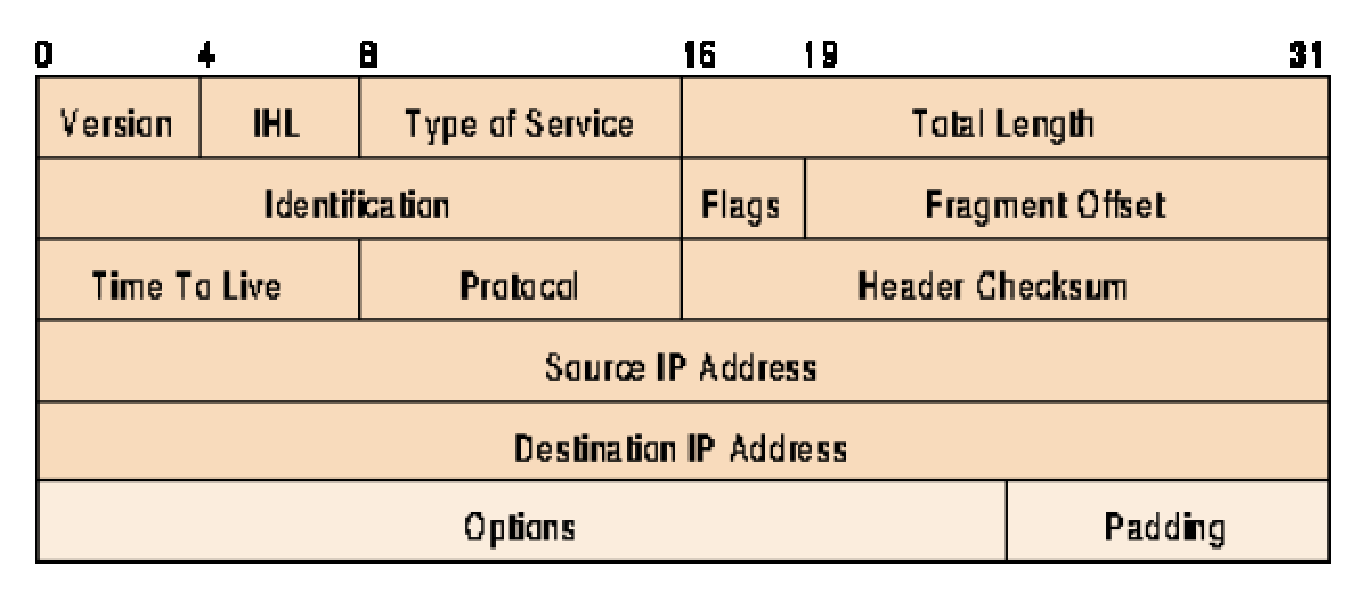
\includegraphics[totalheight=6cm]{iphdr-gif.eps}}
    \caption{IP Header}
    \label{fig:verticalcell}
\end{figure}

Typically size of packets ranges from 100 to 1536 bytes.

Fatesharing: States of a communication are stored only at the end points of a communication. This implies that the connecting devices
do not have to deal with any of the actual contents of packets. This simplifies the design of network. Thus, connection shares it's
fate with the two devices it connects. This is referred to as fate sharing. This is the type of architecture proposed by the end-to-end
argument for network design.


\section{Packet Loss/Corruption}
We discussed two causes of packet loss: congestion and network partitions.
We also reviewed some causes of packet corruption.

\subsection{Congestion}
When a node in a network does not have the processing power to handle
the volume of packets it receives it simply discards excess packets.

\subsection{Network Partition}
When power loss or a hardware/software failure causes a switch to shutdown,
any packets the switch was currently processing are discarded.

\subsection{Packet Corruption}
Packet corruption can occur due to software or hardware error which
causes the packet data to change. Another cause of packet corruption
is electrical charge corruption. This occurs when radiation flips bits
of data in transit or while it is store at a node in the network.

\section{A brief description of working of SMS}
SMSes are limited text messages for cellphones. The messages are limited to 160 characters since
this is a service  piggybacked on an already existing communication method between a tower and a cellphone. Packets already in used for 
alerting a phone about signal reception strength and incoming calls was used for SMS.

\end{document}
